%% History:
% Pavel Tvrdik (26.12.2004)
%  + initial version for PhD Report
% Daniel Sykora (27.01.2005)
%
% Michal Valenta (3.12.2008)
% rada zmen ve formatovani (diky M. Duškovi, J. Holubovi a J. Žďárkovi)
% sjednoceni zdrojoveho kodu pro anglickou, ceskou, bakalarskou a diplomovou praci

% One-page layout: (proof-)reading on display
%%%% \documentclass[11pt,oneside,a4paper]{book}
% Two-page layout: final printing
\documentclass[11pt,twoside,a4paper]{book}
%=-=-=-=-=-=-=-=-=-=-=-=--=%
% The user of this template may find useful to have an alternative to these 
% officially suggested packages:
\usepackage[czech, english]{babel}
\usepackage[T1]{fontenc} % pouzije EC fonty 
% pripadne pisete-li cesky, pak lze zkusit take:
% \usepackage[OT1]{fontenc} 
\usepackage[utf8]{inputenc}
\usepackage{color}
\usepackage{listings}
\lstset{ %
language=Java,                % choose the language of the code
basicstyle=\footnotesize,       % the size of the fonts that are used for the code
numbers=left,                   % where to put the line-numbers
numberstyle=\footnotesize,      % the size of the fonts that are used for the line-numbers
stepnumber=1,                   % the step between two line-numbers. If it is 1 each line will be numbered
numbersep=5pt,                  % how far the line-numbers are from the code
backgroundcolor=\color{white},  % choose the background color. You must add \usepackage{color}
showspaces=false,               % show spaces adding particular underscores
showstringspaces=false,         % underline spaces within strings
showtabs=false,                 % show tabs within strings adding particular underscores
frame=single,   		% adds a frame around the code
tabsize=2,  		% sets default tabsize to 2 spaces
captionpos=b,   		% sets the caption-position to bottom
breaklines=true,    	% sets automatic line breaking
breakatwhitespace=false,    % sets if automatic breaks should only happen at whitespace
escapeinside={\%}{)}          % if you want to add a comment within your code
}
%=-=-=-=-=-=-=-=-=-=-=-=--=%
% In case of problems with PDF fonts, one may try to uncomment this line:
%\usepackage{lmodern}
%=-=-=-=-=-=-=-=-=-=-=-=--=%
%=-=-=-=-=-=-=-=-=-=-=-=--=%
% Depending on your particular TeX distribution and version of conversion tools 
% (dvips/dvipdf/ps2pdf), some (advanced | desperate) users may prefer to use 
% different settings.
% Please uncomment the following style and use your CSLaTeX (cslatex/pdfcslatex) 
% to process your work. Note however, this file is in UTF-8 and a conversion to 
% your native encoding may be required. Some settings below depend on babel 
% macros and should also be modified. See \selectlanguage \iflanguage.
%\usepackage{czech}  %%%%%\usepackage[T1]{czech} %%%%[IL2] [T1] [OT1]
%=-=-=-=-=-=-=-=-=-=-=-=--=%

%%%%%%%%%%%%%%%%%%%%%%%%%%%%%%%%%%%%%%%
% Styles required in your work follow %
%%%%%%%%%%%%%%%%%%%%%%%%%%%%%%%%%%%%%%%
\usepackage{graphicx}
%\usepackage{indentfirst} %1. odstavec jako v cestine.

\usepackage{k336_thesis_macros} % specialni makra pro formatovani DP a BP
 % muzete si vytvorit i sva vlastni v souboru k336_thesis_macros.sty
 % najdete  radu jednoduchych definic, ktere zde ani nejsou pouzity
 % napriklad: 
 % \newcommand{\bfig}{\begin{figure}\begin{center}}
 % \newcommand{\efig}{\end{center}\end{figure}}
 % umoznuje pouzit prikaz \bfig namisto \begin{figure}\begin{center} atd.


%%%%%%%%%%%%%%%%%%%%%%%%%%%%%%%%%%%%%
% Zvolte jednu z moznosti 
% Choose one of the following options
%%%%%%%%%%%%%%%%%%%%%%%%%%%%%%%%%%%%%
%\newcommand\TypeOfWork{Diplomová práce} \typeout{Diplomova prace}
% \newcommand\TypeOfWork{Master's Thesis}   \typeout{Master's Thesis} 
% \newcommand\TypeOfWork{Bakalářská práce}  \typeout{Bakalarska prace}
 \newcommand\TypeOfWork{Bachelor's Project}  \typeout{Bachelor's Project}


%%%%%%%%%%%%%%%%%%%%%%%%%%%%%%%%%%%%%
% Zvolte jednu z moznosti 



% Choose one of the following options
%%%%%%%%%%%%%%%%%%%%%%%%%%%%%%%%%%%%%
% nabidky jsou z: http://www.fel.cvut.cz/cz/education/bk/prehled.html

%\newcommand\StudProgram{Elektrotechnika a informatika, dobíhající, Bakalářský}
%\newcommand\StudProgram{Elektrotechnika a informatika, dobíhající, Magisterský}
% \newcommand\StudProgram{Elektrotechnika a informatika, strukturovaný, Bakalářský}
% \newcommand\StudProgram{Elektrotechnika a informatika, strukturovaný, Navazující magisterský}
 \newcommand\StudProgram{Software technologies and Management, Bachelor programme}
% English study:
% \newcommand\StudProgram{Electrical Engineering and Information Technology}  % bachelor programe
% \newcommand\StudProgram{Electrical Engineering and Information Technology}  %master program


%%%%%%%%%%%%%%%%%%%%%%%%%%%%%%%%%%%%%
% Zvolte jednu z moznosti 
% Choose one of the following options
%%%%%%%%%%%%%%%%%%%%%%%%%%%%%%%%%%%%%
% nabidky jsou z: http://www.fel.cvut.cz/cz/education/bk/prehled.html

%\newcommand\StudBranch{Výpočetní technika}   % pro program EaI bak. (dobihajici i strukt.)
%\newcommand\StudBranch{Výpočetní technika}   % pro prgoram EaI mag. (dobihajici i strukt.)
\newcommand\StudBranch{Software engineering}            %pro STM
%\newcommand\StudBranch{Web a multimedia}                  % pro STM
%\newcommand\StudBranch{Computer Engineering}              % bachelor programe
%\newcommand\StudBranch{Computer Science and Engineering}  % master programe


%%%%%%%%%%%%%%%%%%%%%%%%%%%%%%%%%%%%%%%%%%%%
% Vyplnte nazev prace, autora a vedouciho
% Set up Work Title, Author and Supervisor
%%%%%%%%%%%%%%%%%%%%%%%%%%%%%%%%%%%%%%%%%%%%

\newcommand\WorkTitle{Mobile voting application for Android}
\newcommand\FirstandFamilyName{Radovan Murin}
\newcommand\Supervisor{Ing. Martin Komárek}


% Pouzijete-li pdflatex, tak je prijemne, kdyz bude mit vase prace
% funkcni odkazy i v pdf formatu
\usepackage[
pdftitle={\WorkTitle},
pdfauthor={\FirstandFamilyName},
bookmarks=true,
colorlinks=true,
breaklinks=true,
urlcolor=red,
citecolor=blue,
linkcolor=blue,
unicode=true,
]
{hyperref}



% Extension posted by Petr Dlouhy in order for better sources reference (\cite{} command) especially in Czech.
% April 2010
% See comment over \thebibliography command for details.

\usepackage[square, numbers]{natbib}             % sazba pouzite literatury
%\usepackage{url}
%\DeclareUrlCommand\url{\def\UrlLeft{<}\def\UrlRight{>}\urlstyle{tt}}  %rm/sf/tt
%\renewcommand{\emph}[1]{\textsl{#1}}    % melo by byt kurziva nebo sklonene,
\let\oldUrl\url
\renewcommand\url[1]{<\texttt{\oldUrl{#1}}>}




\begin{document}

%%%%%%%%%%%%%%%%%%%%%%%%%%%%%%%%%%%%%
% Zvolte jednu z moznosti 
% Choose one of the following options
%%%%%%%%%%%%%%%%%%%%%%%%%%%%%%%%%%%%%
%\selectlanguage{czech}
\selectlanguage{english} 

% prikaz \typeout vypise vyse uvedena nastaveni v prikazovem okne
% pro pohodlne ladeni prace


\iflanguage{czech}{
	 \typeout{************************************************}
	 \typeout{Zvoleny jazyk: cestina}
	 \typeout{Typ prace: \TypeOfWork}
	 \typeout{Studijni program: \StudProgram}
	 \typeout{Obor: \StudBranch}
	 \typeout{Jmeno: \FirstandFamilyName}
	 \typeout{Nazev prace: \WorkTitle}
	 \typeout{Vedouci prace: \Supervisor}
	 \typeout{***************************************************}
	 \newcommand\Department{Department of Computer Science and Engineering}
	 \newcommand\Faculty{Faculty of Electrical Engineering}
	 \newcommand\University{Czech Technical University in Prague}
	 \newcommand\labelSupervisor{Supervisor}
	 \newcommand\labelStudProgram{Study Programme}
	 \newcommand\labelStudBranch{Field of Study}
}{
	 \typeout{************************************************}
	 \typeout{Language: english}
	 \typeout{Type of Work: \TypeOfWork}
	 \typeout{Study Program: \StudProgram}
	 \typeout{Study Branch: \StudBranch}
	 \typeout{Author: \FirstandFamilyName}
	 \typeout{Title: \WorkTitle}
	 \typeout{Supervisor: \Supervisor}
	 \typeout{***************************************************}
	 \newcommand\Department{Department of Computer Science and Engineering}
	 \newcommand\Faculty{Faculty of Electrical Engineering}
	 \newcommand\University{Czech Technical University in Prague}
	 \newcommand\labelSupervisor{Supervisor}
	 \newcommand\labelStudProgram{Study Programme} 
	 \newcommand\labelStudBranch{Field of Study}
}




%%%%%%%%%%%%%%%%%%%%%%%%%%    Poznamky ke kompletaci prace
% Nasledujici pasaz uzavrenou v {} ve sve praci samozrejme 
% zakomentujte nebo odstrante. 
% Ve vysledne svazane praci bude nahrazena skutecnym 
% oficialnim zadanim vasi prace.
%%%%%%%%%%%%%%%%%%%%%%%%%%    Titulni stranka / Title page 

\coverpagestarts

%%%%%%%%%%%%%%%%%%%%%%%%%%%    Podekovani / Acknowledgements 

\acknowledgements
\noindent
Placeholder


%%%%%%%%%%%%%%%%%%%%%%%%%%%   Prohlaseni / Declaration 

%\declaration{V~Kořenovicích nad Bečvárkou dne 15.\,5.\,2008}
\declaration{In Košice on Jan 2, 2011}


%%%%%%%%%%%%%%%%%%%%%%%%%%%%    Abstract 
 
\abstractpage

The aim of this work is to design and implement an electronic voting application for the Android platform that will enable people to vote securely from anywhere. The application as a whole is aimed at being compatible with devices from many manufacturers and running different versions of the operating system. The application is also aimed at being localised.



% Prace v cestine musi krome abstraktu v anglictine obsahovat i
% abstrakt v cestine.
\vglue60mm

\noindent{\Huge \textbf{Abstrakt}}
\vskip 2.75\baselineskip

\noindent
%Ľudia začínajú čím ďalej tým viac integrovat mobilné zariadenia do ich každodenného života. Uľahčuje to život, odbremeňuje nás to od stáleho cestovania a zvyšuje produktivitu.
 Cieľom tejto práce je navrhnúť a naimplementovat aplikáciu pre elektronické hlasovanie pre platformu Android, ktorá umožní ľudom hlasovať bezpečne z akéhokoľvek miesta. Celá aplikácia je zameraná na čo najvačšiu kompatibilitu medzi rôznymi výrobcami a verziami Androidu a jazykovú prenositeľnost.
 

%%%%%%%%%%%%%%%%%%%%%%%%%%%%%%%%  Obsah / Table of Contents 

\tableofcontents


%%%%%%%%%%%%%%%%%%%%%%%%%%%%%%%  Seznam obrazku / List of Figures 

\listoffigures


%%%%%%%%%%%%%%%%%%%%%%%%%%%%%%%  Seznam tabulek / List of Tables

\listoftables


%**************************************************************

\mainbodystarts
% horizontalní mezera mezi dvema odstavci
%\parskip=5pt
%11.12.2008 parskip + tolerance
\normalfont
\parskip=0.2\baselineskip plus 0.2\baselineskip minus 0.1\baselineskip

% Odsazeni prvniho radku odstavce resi class book (neaplikuje se na prvni 
% odstavce kapitol, sekci, podsekci atd.) Viz usepackage{indentfirst}.
% Chcete-li selektivne zamezit odsazeni 1. radku nektereho odstavce,
% pouzijte prikaz \noindent.

%**************************************************************

% Pro snadnejsi praci s vetsimi texty je rozumne tyto rozdelit
% do samostatnych souboru nejlepe dle kapitol a tyto potom vkladat
% pomoci prikazu \include{jmeno_souboru.tex} nebo \include{jmeno_souboru}.
% Napr.:
% \include{1_uvod}
% \include{2_teorie}
% atd...

%*****************************************************************************
\chapter{Introduction}

\paragraph*{}
Voting is a delicate matter. Whoever the voter is, he or she usually wants to vote as transparently and freely as possible. In most cases this is achieved by strict rules which often make it necessary for the voter to be physically present. But what about the one member of the board who is always traveling? What about a member of a council that is stuck in a traffic jam on the way to the council hall? \\
In today's world we are witnesses of a process that is merging two devices into one. The PDA - Personal Digital Assistant and the cell phone. This means that more and more people carry in fact powerful computers in their pockets that enable them to perform a lot of tasks without the need of being at their desks. It also enables a person to vote safely and easily while he is unable to attend a meeting in person. 

%*****************************************************************************
\chapter{Description of the problem and goals}

\section{Description}
The main idea is to have a system that enables people to vote electronically without the need of having to move to a voting machine. This should quicken the whole process of voting and eliminate the need of error-prone human vote counters and provide. The problems of such a system can be divided into six areas:
\begin{enumerate}
\item Authentication and registration- determining whether or not the person behind the user name and password.
\item Data Transfer and device security - ensuring that the devices communicate in a safe and efficient manner.
\item Voting - 	emulating the voting process so that it reflects real life voting, designing safe storage of the results.
\item Result Presentation - presenting the voting results in an easy and accessible manner.
\item Device compatibility - making the resulting application to run on a large number of devices.
\item Ease of use - the voter is aimed at an average user, the manuals and design must reflect that.
\end{enumerate}

This work is based on Jakub Valenta's bachelor's thesis\cite{bakalarkaJV}. In this thesis, he created a fully functioning voting server,the part running on a personal computer and counts the votes, and a J2ME client, the part with which the voter actually votes. Now, in the conclusion of his bachelor's thesis , Jakub Valenta \cite{bakalarkaJV} states, that the ever changing and manufacturer specific implementation of Java ME, configuration CLDC and MIDP specification is the biggest obstacle in implementing his software on a larger scale.  The aim of this work is to overcome this shortcoming and create a new application that will communicate with a server based on his work. 

\subsection{Authentication and registration}
The number of voters makes it tricky to register. The goal here is to make the registration process as quick and as unambiguous as possible.
\subsection{Data Transfer and device security}
When voting on a delicate matter, privacy and voter intent cannot be tampered with by for example a man-in-the-middle type attack. The voter has to be sure that his vote has been received without change and in the case if a secret ballot, unseen by a third party. \\
Next, the nature of how the Android platform enables parts of an application to launch within another application. The resulting "app" will have to deal with this.\\
Another thing is physical security. The cell phone will never be safe from this perspective. People often leave them at hotels, public restrooms, they are often the target of small theft. Because of this fact, the phone application will have to be protected from unauthorized use. A more detailed analysis of this issues is in the chapter Analysis, section Security\ref{sec:security}.   \\
\subsection{Voting}
The voting process is described in Jakub Valenta's work \cite{bakalarkaJV} . The process is based on real life voting where people first see the question and answers. Then they choose their answer of choice and send their vote. The system acts just like a human vote counter and counts up the votes and publishes them on the web or wherever it is suitable. 
\subsection{Result Presentation}
What purpose the voting would serve if the people wouldn't be able to see the results? The aim in this category is to present the results in an easily accessed human readable form.
\subsection{Device compatibility}
As stated in the introduction in this chapter, mobile devices tend to have different implementations of even standardized APIs(Application Programming Interface). This makes implementing one application for all devices impossible. Therefore, another goal is set. Multiple versions of the application. Each version will work one one platform. By starting at the most widely used platform and continuing to the second, third...etc, it is possible to cover a rather wide range of devices.
\subsection{Ease of use}
The people that will be using this piece of software will not be IT professionals. This has to be taken in account when creating manuals and installation packages.The main aim is to make the software so easy to use that the average user will be able to benefit from it.
%\subsection{Android} 
%


%Je to vobec nutne? vsetko je rozobrane



%Toto skor do analyzy
 %The voting process itself does not have to be changed, however it is not necessary nor desirable to have such little features on an Android device. If the voter is a not present at the a meeting or congress , it would be difficult for him to know the details of the event and the people involved in it. 


%Therefore the voting ticket has to be altered.\\
%Since the aim of this work is to create a voting application, testing part that is meant for school use will not be altered. 



\subsection{Already existing systems}
Applications for the Android platform are distributed with the Android Market tool \cite{MarketAnd}. Presently, there are only a few "apps"  that offer voting. All of which use an unsecured connection and use a server that has unknown security settings. Also none of these "apps" offer a J2ME application for a feature phone. \\
Apps for mobile voting (Android Market, state from 21.1.2011): 
\begin{itemize}
\item "Handy Poll" by Marc Tan \cite{HandyPoll} \\
The application Handy Poll is, as the name suggests, used mainly for polling. As an example I would state a situation where a student of psychology needs input data from a lot of people. He/She creates the questions and responses. Then, people see the questions and can respond to them without authentication.
\item "android mobile voting" by Dare Labs for Sony Ericsson \cite{DareLabs}\\
Presently not functional. Advertised to be safe. I could not get it to work. Although the company website \cite{DareLabsWeb} is claiming that the application is fully functional.
\end{itemize}



\section{Goals}

The goal of my thesis is to enhance the voting system from Jakub Valenta's\cite{bakalarkaJV} thesis in such a way, that it will enable voting from a mobile device running Android\cite{whatisAnd} and thus broaden the spectrum of devices supporting this software. My aim is to make use of the larger capabilities that an Android device provides in comparison with a simple phone and enhance the user experience and create a baseline which future developers for different platforms can use. 

\subsection{Android side}
The Android application is to be written from scratch in Java for Android (Dalvik VM\cite{DalvikVM}). It will enable the user to vote securely, provide the user with basic information about the candidates or choices - e.g. age, occupation, few words about ballot choices. The Android application will also be able to view the results of a closed question. In order to maximize the number of people able to use this software it will also be localized into several languages.

\subsection{Server side}
The main goal here, is to increase the amount of information the server provides about the question and itself. without compromising the compatibility with the J2ME application. Next, is to implement a secure way of communicating with the clients so that the security will no longer be reliant on Wi-Fi encryption. Another goal is to be able to differentiate between clients connecting from the local network and users connecting from the Internet and enhance the authentication.



% For practical application this will have to be changed. The server will also have to be changed to be more election orientated. That means that support for election details and result sending will have to be added. 

\subsection{Feature phone side}
The feature phone application will remain compatible with the edited server. \\

\subsection{Summary}
In summary the aim of this work is:

\begin{itemize}
\item To extend the capabilities of the server so that it will be able to communicate with the new device.
\item To design and create a functioning Android voting application.
\item Maintain compatibility with the existing J2ME client with minimal editing.
\item Make the system user friendly.
\item Ensure that the voting is safe.
\item Ensure that stored voting credentials are safe after device theft.
\item Provide the user of the Android application a choice of language: English, French, Slovak and Czech. And create the application in such a way, that facilitates implementing new languages.
\item Minimize the risk that the Android application will not work in future releases of android by using best practices for Android applications.
\end{itemize}
%THE SECTION ABOVE HAS BEEN CLOSED FOR REVIEW
%*****************************************************************************
\chapter{Analysis}
\section{Vision}
This electronic voting system will be based on the existing work of Jakub Valenta/cite{bakalarkaJV} and will enable people to vote electronically without the need of a person. This will eliminate the problems of counting errors and provide a new degree of security. The system will be primarily designed for group decision making where the majority decides but it will be also usable for candidate voting. The whole voting process will take place from a mobile device. The system will be highly portable and usable in an international environment.
\section{State of the software at the beginning}
\subsection{Overview}
\paragraph{}
The system in the received state was fully functioning and able to run the ballot with a J2ME device.(This was tested only in an emulator).The system enabled the user to vote in a very simple way. The user chose to create an election, inputed the questions and possible answers, chose the threshold percentages for a successful voting event, created voters with a simple form and started the voting process. The voters then could vote via their cell phones. After some time the voting is stopped and the server displays the results in the results tab. \paragraph{}
The communication was handled by HTTP. Jakub Valenta\cite{bakalarkaJV} states that he chose this protocol because of the guaranteed delivery it provides. But while HTTP is a reliable protocol, it is the TCP layer that provides this functionality. The benefits as I see them are mainly that it is a standard and HTTP parsers are easy to use and already implemented in Java. On the other hand, the question whether it is not too much of a load for a Java ME enabled device to parse such requests arises. But that is out of the scope of this work.


\subsection{Negatives}
Suppose there is a ballot question such as this: "Do you agree with proposal no. 22?" The purpose of mobile voting is to be able to vote from wherever the voter is right in the moment and it is possible that he will simply not know the details behind such proposals because he is not physically present at the meeting. This is a problem when using the current system as there is no simple way of providing the details about the question at hand.\\
Another negative is that SSL is not implemented in communication with the server. This means that anybody who has access to the Wi-Fi through which the voters vote can see all data en route between the devices. And although the connection between a cell phone and the BTS\cite{whatISBTS}  is encrypted, this encryption has been proven to be weak\cite{GSMCypherWeakness} and breakable in real time. This fact  prevents the use of a cell phone network as a data carrier without encryption on a higher network layer. What is worse than seeing the data is changing them. When using an open network (no access control) virtually anyone with the right software can alter the data.\\
As stated previously, in spite the fact that the majority of the currently sold cell phones support J2ME the application is unlikely to run on most of them because of compatibility issues.\cite{bakalarkaJV}

\subsection{Positives}
On the other hand the work has it's positive features. The fact that the voting was made so simple made running it on a limited device smooth and without problems. The installation was without problems and was quick. The user interface was very comfortable and straightforward. This enabled very easy initial setup without a tutorial.\\
The communication protocol is very efficient and therefore enables the use in areas without 3G signal. (it will even work swiftly with a basic GPRS connection. Documentation was excellent. All in all, the application does what it needs and does it well.
%Todo Po vacsej analize bakalarky viac pozitiv


\section{Server}
A server is the part of the system that counts the votes, listens to connections and authenticates people. As this role is a practically a single point of failure, it needs to be well designed, and also well implemented. When creating an application such as this is the issue of the number of concurrent connections and operations. This system is designed to be used in a small to medium sized environment with  a maximum of 200 concurrent connections. A larger number would require expensive hardware equipment and/or load balancing. Load balancing will not be used or implemented. The server is also responsible for advertising its presence on the local area network, offer a means of voter registration and providing simple information about how to connect. The first part is solvable by using a UDP\cite{whatIsUPD} broadcast\cite{whatIsBroadcasting}. In short, this will send a datagram to all the computers within a network with the information needed to achieve a connection as well as a friendly name of the server. I chose UDP broadcasts because UDP is unreliable, meaning the sender does not wait for a response. Also this is the standard way of sending adverts through the network. The second part is solvable by multiple ways. First, and this is how Jakub Valenta's system works, the user creation is strictly local, and the administrator,the person in charge of creating the elections, creates the users manually. This requires the voters presence and  it is painfully slow (imagine 200 people before some event standing in line to enter their passwords). What would be better is, to create a web page with a simple form where users would input their names and login credentials. A script would then aggregate this data in a file, possibly an XML file for simplicity, and then another program would be used when verifying the voters identity. Although this would not mean the disappearance of the 200 people lines, it would fasten the process significantly, as only a personal number would have to be verified. The third problem, the info and registration web page, is solvable by implementing a simple web server into the present server software, by using a lightweight HTTP server(Apache for example)  in concurrency with the server software or using a small web server library. Using an external web server - such as Apache, IIS, nginx, would be very easy from an implementation point of view, however for the end user the installation and configuration of any of these servers would be a hardly overcomable obstacle. Implementing a new server would be a waste of time and effort as there are plenty of libraries with light-weight HTTP servers. For these reasons I decided to use a small HTTP server library. I have previously mentioned a personal number. This number or alphanumerical combination will be used to verify the identity of the registered user. It could be his ID Card number, Drivers license number anything person bound. Because it will be possible to vote from the Internet, a new system of verifying the connecting user origin will be needed. The system is necessary when the jurisdiction or some other agreement stipulates that the voter is to be present at a specific place. The Wi-Fi's limited range ensures this. Because the two possible mobile devices will be connected, the server will have to support multiple types of connections.

\section{Client}
The client is the part of the system that provides an interface for the voter to log in, vote and check the results. This part should be easy to use, lightweight and most importantly compatible with a lot of devices and safe. The safety of the mobile device is for a larger analysis and has a dedicated section that follows this one. The problem of user friendliness is really a matter of designing the application to behave consistently with the operating system. Explanation: an Android user is knows how Android applications usually work and expects this one to behave in this manner. It would be very confusing to use the same design principles for an iPhone, which has one useful hardware button, and an Android phone which has at least four. The next problem is being lightweight. The application is running on a very limited device. Limited in computing power, bandwidth, memory and electric power. In the context of our application, computing power is not really an issue as no business logic is done on this end and computations are not very demanding. The bandwidth is also not a big concern as the data that is send is plain text and as such is not very large. The main problem that we need to combat here is power drainage and memory consumption. Every open connection on a cell phone lowers it's power levels considerably. The phone will therefore have to use the connection as little as possible and close the connection after every request. As conference events and voting can involve people that speak multiple languages, the mobile application should be designed to be easily translatable. This is done by using external strings when making any writings in the applications.\\
Platform specific analysis:
\subsection{Feature phone}
The feature phone is the most limited of all mobile devices. It runs a very basic implementation of Java ME, has very little computing power and no multitasking capabilities. This added up means, that the client has to be very basic.
\subsection{Android device}





The main problem concerning the Android system is its speed of development and different versions that are currently released. It was stated previously that Android is mostly forward compatible, but the as the version is higher the framework has more and more functionalities that make some of the programming unnecessary. The question here is the choice of the version on for which the application will be written. The distribution of versions are in the figure below.

 As an application was already written for the J2ME platform the next logical choice is Android. The benefit of Android\cite{whatisAnd} is that while Java ME implementations may vary, Android is mostly consistent and a piece of software written and tested on one device should work on another. Forward compatibility is not guaranteed but as the changes are mostly additive, it is highly probable. \cite{goodevpi}


\begin{figure}[h]
\begin{center}
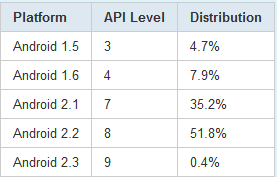
\includegraphics[scale=1]{figures/VersionDistribution.PNG} 
\caption{Version Distribution of Android \cite{goodevver} from http://developer.android.com/resources/dashboard/platform-versions.html retrieved on 22.1.2011  }
\label{fig:versions}
\end{center}
\end{figure}


As it is clearly depicted in the table the prevalence of Android 2.1 and higher is overwhelming. Therefore Android 2.1 was chosen to be the minimum version supported by the application.
 	


\section{Security analysis}
\label{sec:security}

As it was stated earlier, mobile devices are susceptible to a number of threads. 
\begin{enumerate}
\item Physical theft
\item Man in the middle attack
\item Malicious applications posing as legitimate software in order to trick the user into giving away his login credentials.
\item Malicious servers %Toto asi presunit do vlastnej state
\item Rooted device
\end{enumerate}
\subsection{Physical theft}
Physical theft poses a risk that the stored login information in the device. While the most obvious solution would be not to store login credentials on the device. This would be inconvenient for the end user. Therefore a better solution would be, to request a master code upon every application launch. Another possibility for the software would be making an IMSI number check and in an event of a different SIM, or no SIM being inserted into the device, the app would wipe all user data on launch. 
\subsection{Man in the middle attack}
A man in the middle attack is a common attack where the attacker has access to the transfer medium (in our case air). The attacker can then see the data being exchanged or, what is worse, alter it. In order to protect against such an attack the whole communication has to be encrypted, preferably by SSL. This, along with a Certificate signed by a trusted authority should ensure that the application will always know if the communication is being tampered with. Proper training manuals will have to warn the users about the dangers of unsecured connections.
\subsection{Malicious software}
The graphics interface of the application can be replicated and the user made to believe that he/she is entering his login credentials to the real application. This problem can be avoided by signing the application, and proper user manuals.\\
Next, a malicious program can try to copy stored data of the voting app. This problem is addressed by using a private storage mechanism provided by Android. \cite{storageAnd}
\subsection{Malicious servers}
Because this software is open-source, anybody can alter its behavior and run it. This creates a potential security thread where users could connect to a false server that is advertising on the same local area network. Here the users would give their login credentials in false belief that they are giving them to a legitimate server. In reality they would be disclosing them to a third person who could then use them to login to the original server and vote on their behalf. The same problem goes for the server information web page and registration web page. The advertising issue can be solved by careful network settings which are discussed in the deployment section. The web page problem solution is identical to that of the Man in the middle attack problem solution.
\subsection{"Rooted" device}
Normally, an application run on an Android device cannot obtain root access to the device. This ensures that application security is kept intact. Hidden application per application data is protected from being read and altered by the wrong application. This, however, is not true when running a "rooted" device. The applications on that device can obtain root access and read sensitive data. To combat this risk, the stored password will have to be encrypted, and the user warned about the risks of having root access.


\section{Business process model}
The business process model was created by Jakub Valenta and it depicts the process how voting is held without the use of an electronic voting system. \cite{bakalarkaJV} \ref{fig:businessMOD}

\section{Requirements analysis}
The requirements analysis is comprised of the requirements the system must achieve to be complete. The system must support all requirements concerning voting from Jakub Valenta's thesis and in addition, those stated further in this section.
\subsection{Functional requirements}
\paragraph*{Server}

\begin{enumerate}

%\item  The system must support two-factor authentication.
\item  The system will provide the user with a wifi-only mode and a fully mobile mode.
\item  The system must provide detailed information about the questions.
\item  The system will present connection information on a simple web site.
\item  The system will enable the users to vote publicly. \cite{bakalarkaJV}
\item  The system will enable the users to vote secretly. \cite{bakalarkaJV}
\item  The system will enable new user registration. \cite{bakalarkaJV}
\item The system will evaluate the results of the vote.\cite{bakalarkaJV}
\item The system will be able to present the results.\cite{bakalarkaJV}
\item The system will guarantee the explicitness and the indubitability of the vote. \cite{bakalarkaJV}
\item The system will ensure persistent storage of data. \cite{bakalarkaJV}
\end{enumerate}
\paragraph*{Client}
\begin{enumerate}
\item The application must enable the voter to login. 
\item The application must enable the voter to view question information.
\item The application must enable the voter to view the results of a closed vote. 
\item The application must enable the voter to vote.
\item The application must provide basic safety guidelines when first run.
\item The application must remember the connection information and login data to multiple servers.
\item The application must warn the user when using a non-secure connection when security is medium.
\item The application must enable multiple connections to various servers.
\item The application must notify the user when a question has been finished.
\end{enumerate}
\subsection{Non-Functional requirements}
\paragraph*{Server}
\begin{enumerate}
\item  The system must support both HTTPS and HTTP connections.
\item The system must be compatible with the current J2ME client.
\item The system must be able to communicate swiftly with any mobile connection.
\item The system must be secured from being tampered with by unauthorised personnel.
\end{enumerate}
\paragraph*{Client}
\begin{enumerate}
\item The application must use as little power as possible.
\item The application must be usable on a variety of screen densities and sizes.
\item The application must be usable on a device with or without a touch screen.
\item The application must be easy to use and fast to learn.
\item The application must provide an easy way to add a new language.
\item The application must store the user's login information in such a way that other applications will not be able to access it.
\end{enumerate}
\section{Use Cases}
The use cases describe the probable interactions with the system and how the system will react to them. They are fully described in the UseCases file enclosed with the thesis. The user can choose the server he wishes to log into, then can display the details of the questions and vote on them. Time and the Android system itself play a minor role in the use cases because of how Android manages memory. For the sake of simplicity application components are represented as one activity. Further information concerning the use cases are in the 



\begin{figure}[h]
\begin{center}
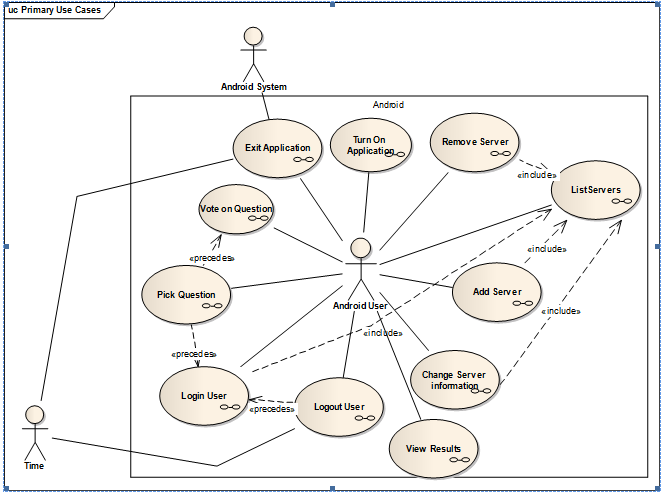
\includegraphics[scale=1]{figures/AndroidUCs.PNG} 
\caption{Use cases for the Android Application}
\label{fig:Use Cases}
\end{center}
\end{figure}
%\section{Domain Terminology}
%This aim of this section is to provide a clear understanding of the terminology used in this work. Most of the terms are intuitive and easy to understand however there are some that need clarification.
%\paragraph*{Activity and Application}
%In this work the work application is referring to an Android "App" written in Java for the Dalvik VM. It is often hard to distinguish between what is an application and what is an activity. In simple terms an application consists of a number of activities each aimed to fulfil one task.
%\paragraph*{User}
%The user is, of course, the person who makes use of the system. In this work, two types of users are distinguished. The voter and the administrator. The voters role is simple, login to a server and vote. The administrator's role is a little more complex, input the questions, add voter accounts and open/close voting. As the administrators part has been analysed in the previous work, it is not given much notice here.
%\paragraph*{Question and Response}
%A question is a request for information concerning a subject and aimed at the user. A response is the answer to such a request. In the effort of simple processing the voter is given a set of responses from which he can choose. The questions have no right or wrong answers, they are polling questions. Every question has a details field which enables the voter to see the full wording of the %\paragraph*{Server}
%A server is an application that listens for a connection. For the application a server is a collection of data that is needed for a successful 
%\paragraph*{View}

%\paragraph*{Service}
\section{Domain Model}
This model describes the various relationships between objects in the problem domain. It is based on the Jakub Valenta's domain.
This model describes how the client side on android sees the problem. The model is similar to that of the original, but takes to account that the use of this system will be purely for voting. 
\subsection{Server}
The server domain model represents how the server sees the objects involved in voting. A full description is here \cite{bakalarkaJV} but as a quick reference the main purpose of the entities are briefly described.
\paragraph{Voting Entity} 
The voting entity represents a vote event. It's attributes are isSecret used so signal if users vote secretly and minVotes - the minimum turnout of the event to be valid.
\paragraph{User} 
The user entity represents a user within the system. It's attributes are self explanatory.
\paragraph{Vote}
This entity is the ballot. It is the form that voters fill out and send to the voting commission.
\paragraph{Question}
The question entity represents one question on the voting ticket. Its attributes are maxWinners - the number of winners, minPercent - the minimum percentage to be successful and text - an XML representation of the question and answers. 
%Dopis detaily o otazke
\subsection{Android}
From a clients perspective the domain model is a little different. It does not concern itself with the details about the voting event and does not participate in results calculation. On the other hand, the client has to deal with being connected to multiple servers and save users.
\paragraph{ServerData entity}
The server entity represents the a real server application running on a computer somewhere on the Internet.Its attributes are the settings that the client needs to create a connection to a server. It consists of an IP address or host name of the target server, the port through on which the server is listening. It also has a friendly name.\\
Next the server contains, the login data for one specific user. The password is encrypted. The user is  an authorised user in the system that is created on the server. \\
The whole entity has a unique id that identifies it in the SQLite database.
\paragraph{QuestionData entity}
The questionData class serves as a container for the question text and the corresponding details and as a container for the possible answers. The states of the question here is quite similar to those on the server but the NOT\_SET attribute is meaningless and therefore left out. The chosenAnswer attribute is the presently chosen answer that will be sent The other attributes are ANSWERABLE, meaning the question can be answered, and FINISHED. A finished question is open for result viewing. 
\paragraph{Answer entity} 
This represent the possible answer for the question that is stored on a server. Its attributes are percent and text. The former represents the percentage of people that voted for this question, this is only found when a question is in the "FINISHED" state, and and the latter represents the question text.





\begin{figure}[h]
\begin{center}
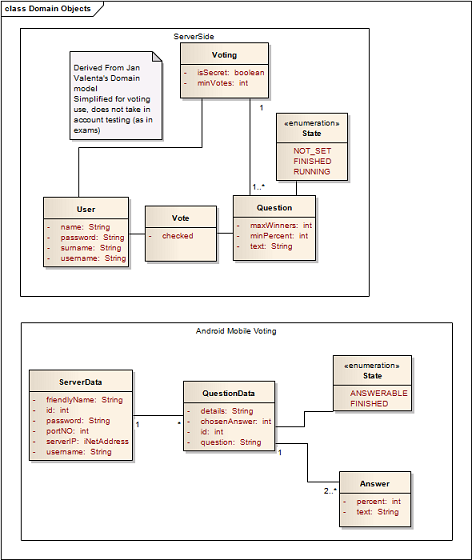
\includegraphics[scale=1]{figures/DomainObjects.png} 
\caption{Domain Model of the System}
\label{fig:Domain Model}
\end{center}
\end{figure}



%***************************************************************************************************************************

\chapter{Design}
The design of the "Mobile Voting System" is the original design of Jan Valenta which was extended in order to add functionality.
\section{Communication}

Presently, the communication is handled by the HTTP protocol. This protocol has, in my opinion, and advantage in being standardized and so it facilitates implementing the communicating part of the application. The protocol, however, is not safe. It sends data as open text and that is not acceptable for this kind of an application.\\
 Therefore, Android applications will send a special "Hello from Android" message in the message body. The server then will either send a "426 Upgrade Required" code, which will indicate that the client has to try again using HTTPS, or will accept the connection without encryption. The message will have and optional port number, if the server is using a non standard port for secure connections. This behavior will depend on the security settings on the server side. \\
  The feature phone will continue to use HTTP as altering it's programming in such a degree is beyond the scope of this thesis. If the security will demand it, the server will reject any non-encrypted communication attempted through a mobile network. The connection termination will be preceded by a "419 LAN REQUIRED" code. Feature phones will still be able to connect through a Wi-Fi connection. Provided that the Wi-Fi is protected.\\
 
This differentiation will be possible because of the new IP checking mechanism that will be added. When a client connects, the server will perform an IP check to determine whether the client is connecting from the local network or not. The easiest way to perform this check is to see if the IP address is from the private subnets. As a packet with a private IP cannot survive on the Internet(it is discarded by the first properly configured router), it is safe to assume, that such a packet came from the local network. The reason why I perform this check is to ensure that the voter is physically present at the voting site when the legislature of some other rules require it. VPN technology is to be dealt with on the operating system level.\\

It is crucial that the client will not send the password when the communication is to be encrypted. Therefore, the first "hello" message has to be without a password. If a faulty client implementation sends the password unencrypted in this first hello message the server will invalidate the credentials of that user and add a log about it.\\

Data in HTTP answers will be sent in the XML format created by Jan Valenta. A new tag will house question details. Furthermore a new DTD will be created to form the XML data that will be sent when election results will be requested.

\subsection{Summary of codes used in communication}
Original\cite{bakalarkaJV}
\begin{itemize}
\item 200 Request success
\item 400 The request was not understood by the server. The server understands only GET and POST request.
\item 401 Authentication credentials bad.
\item 403 Authentication credentials required and not present.
\item 404 Nothing to send.\\
\end{itemize}

Extentions
\begin{itemize}
\item 426 Use HTTPS protocol
\item 419 Local area connection required
\item 466 Security was compromised by sending an unencrypted password.
\end{itemize}
\section{Server side}
\subsection{Minor Changes}
The server GUI will have some minor changes from it's original version. The questions table will be enhanced with a new column called "Question Description". Next, a new security setting dialog will be added when creating a new election event and it will now be possible to use custom TCP ports in case the server will  have those ports blocked by a web server, or some other application. The persistence layer will mostly remain unaltered apart from the new "details" attribute.


\section{Android side}
The android application will be designed with best practices for the platform in mind. It will be build using the MVC model\cite{whatIsMVC}.

\subsection{Graphical User Interface (GUI) - View}
The application will have a minimalist user interface that will enable to use touch screens with ease.The main screen will consist of a list of servers that were added in advance. After choosing the desired server and a successful connection the application will view possible questions. Again in the of a list. The user will then choose a question he wants to view. Here, the application will behave in three different ways. First, it will normally display question details, and possible answers, second behaviour is to display the question results - as an ordered table when the question is closed and results published, third is to inform the user that he has already answered, and the results are not yet available.  \\
Possible answers to a question will be displayed as  buttons. After the desired answer is selected, the user will be able to send his response by long pressing the question button. The send button is hidden in order to reduce the risk of accidental sending. \\
When designing the GUI, the possibility of a third person being able to look at the devices display has to be taken into account. The passwords are never shown as text, therefore no risk exists in that somebody will see the password. However, there is a risk that someone will, on purpose or by accident see what answers are highlighted. One secure way of displaying the chosen answer is, of course, not to display them at all. This, however, poses more dangers than benefits. It introduces uncertainty for the voter about which answer they have chosen as touch screens are not very precise. A compromise is, that the choice will be highlighted for only a few second after the user has made his choice. With this in mind the user inteface will print out a small discrete message with the chosen answer for a shot amount of time after choosing the answer. \\
Every action will be confirmed by a notification.\cite{bakalarkaJV}	

\subsection{Persistence}
The application will need to store user login credentials, server information and temporarily store questions and related data. The data that needs to be saved even after a system reboot - credentials and server info, will be in a private SQL database that Android provides for every application. The database,on an non-rooted\cite{whatIsRoot}  phone,  is completely private and no other applications can gain access to it. If the device should be stolen and rooted, the password encryption should offer the legitimate user time, to reset his password and prevent any damage. \\
Another problem is, what will happen when the device receives a phone call or switches to some other application \cite{bakalarkaJV} at some point during the voting process. Because Android typically runs on low memory devices, it often simply kills an application when it needs more memory. This however, is not without saving the data structures belonging to that application first. The user notices nothing. This is entirely done by the Android system.\\

\subsection{Communication}
As it was stated in the previous section, Android kills an application when it runs out of memory. This can happen to the voting application too. When this happens, the connection would normally be lost. The platform thinks of this and provides a component called "service". The service runs independently from the graphical interface and has a lower "to kill" priority when memory shortage occurs. \\

Because of this, the communication part of the application will be in the "service" component and will dynamically bind with new views in case the former got killed. The subsystem will have to be efficient and conserve battery as much as possible. It will also have to take into account the specific problems of a portable device - sudden loss of connectivity \cite{bakalarkaJV}. 




	
%*****************************************************************************
\chapter{Implementation}
Implementation is the part of a software development process where the design becomes a real program. This step involves choosing the programming language, writing code and compiling.

\section{Tools}
\subsection{Programming language}
The programming language defines some key characteristics of the final product. Some languages offer great optimization and some are good at being portable across many platforms. The language chosen for this project was Java and Groovy\cite{whatIsGroovy}. While the application could have been written in any other language, I chose Java as the programming language to implement it. First, concerning all the programming languages I know, Java is my most preferred because of the vastness of it's libraries, secondly Java is platform independent and that means that the time intensive task of recompiling the program for different platforms is removed. The third reason is because the base program was already implemented in Java and Groovy and a complete rewrite would be pointless. In my work, I only used Java and the reasons for using Groovy in some parts of the program are discussed in Jakub Valenta's bachelor's thesis\cite{bakalarkaJV}.

\paragraph{Java platform}
A Java platform is a specific set of standards that enable Java written code to be run. \\
As my predecessor I have chosen to use the Java SE\cite{whatIsJavaSE} platform. Java SE is a general-purpose platform and is well suited for this type of project.

\paragraph{Android platform}
Android applications can be written in either Java or C/C++. Programming applications for this platform in C/C++ however, has a number of drawbacks. One of which is bad portability. I is unlikely that an application written in this way will be very portable. For this reason I decided to use the recommended Android platform, which uses the Java programing language. This also made implementing the whole system easier I was using only one language, albeit different platforms.

\subsection{3$^{rd}$ party libraries}
By a  3$^{rd}$ party library I mean a piece of compiled code that is used as a pre made solution for common problems that  is not included in the original collection of Java SE libraries or Android libraries.
\paragraph{XML Pull\cite{xmlpull}}
This is the only third party library which is used in the implementation. While a part of the standard Android library suite this is not a part of Java SE. This library XML serialization and does this in a much simpler way than the traditional Java SE serializers. An example of use in my implementation is the method providing a fall-back generation of the registration web page.\\
\begin{lstlisting}
      public String makeIntroPage(String IP, int port) throws XmlPullParserException, IOException {
        XmlPullParserFactory factory = XmlPullParserFactory.newInstance(
                System.getProperty(XmlPullParserFactory.PROPERTY_NAME), null);
        XmlSerializer serializer = factory.newSerializer();
        String xml = new String();
        StringWriter os = new StringWriter();
        serializer.setOutput(os);
        serializer.setPrefix("", NAMESPACE);
        serializer.startTag(NAMESPACE, "html");
        serializer.startTag(NAMESPACE, "head");
        serializer.startTag(NAMESPACE, "meta");
	}
\end{lstlisting}

\subsection{User Interface}
\paragraph{Server}
The GUI of the server application is implemented using Swing and Groovy. As stated beforehand Groovy is was not used in this project but rather inherited. Therefore, it will not be discussed. Swing is a great toolkit for creating a simple GUI such as used in this project. To design the user interface I used the standard design tool that comes in Netbeans.
\paragraph{Android}
The Android framework does not enable the developer to use any other GUI framework other than it's own toolkit. The icons for the project are from an open source icon library\cite{iconsource}, edited in MS paint when needed.

\subsection{Cryptography}
Creating a TLS\cite{tls} connection requires the server, the listening part, to have a digital certificate. For testing and development purposes a self-signed certificate was sufficient.To generate this certificate, and all other default certificates used in the application I used OpenSSL\cite{openssl}.

\subsection{Persistence}
\paragraph{Server} The persistence tools of this side is documented in Jakub Valenta's bachelor's thesis\cite{bakalarkaJV}.
\paragraph{Android}
For persistence of the Android application data a SQLite\cite{sqlite} database was used along with "Shared Preferences"\cite{storage} mechanism. The SQLite database is used for structured data - the server information, and the latter,"Shared Storage" is for storing primitive unstructured data.

\subsection{Used integrated development environments (IDEs)}
There are a number of powerful IDEs to use with Java. For this project I have selected to use Netbeans for the Java SE part and Eclipse for Android. Netbeans was chosen because I had good knowledge of this tool and was confident with it's use. Eclipse was the recommended IDE by Google to develop Android applications. Both these tools were are very intuitive and pleasant to work with. 

\section{Server}
The server is a desktop applciation implemented in Java SE.
\subsection{Prologue - information/registration server}
The Prologue server is the implementation of a voting information and registration server defined in the design chapter. It is a part of the application. The server is implemented using a standard "HttpsServer" java class. This class provides basic request handling. Every request is passed to a handler class. There are two handling classes that this server uses the "registeringHandle" and the "providingHandle". The former has voting registration enabled, while the latter only provides the information necessary to connect with a mobile device.
\paragraph{Connections and encryption}
Clients can only connect to Prologue using a TLS\cite{tls} connection. The connection uses certificates that are used in the handshakes. Java enables the use of a number of certificate formats. First, a Java keystore format was used but then was dropped in favor of PKCS12\cite{pkcs12}. The PKCS12 format has the advantage of being more user friendly and more widespread. The user friendliness comes from the fact that the PKCS12 format is the only standard format that enables private key storage.
\paragraph{Web pages}
The server on its start fetches all files named like "index_[language-code].html". The language-code is the same as the codes in the Accept-languages\cite{httpHead} field in a HTTP request header. The reasons for this will be discussed later on. These pages are parsed and the relevant information such as server IP addresses and ports are added to them. A special "<--PUBLIC_IP-->" and "<--PORT-->" tag denotes the place where where information should be placed.  This web page then serves a the home page providing the registered users all the necessary information needed for the actual connection. When the system does not find any index file that could be used as a main page, then a hard coded one is used as a fallback. The registration page is a simple form page that sends the relevant data to the server via the POST HTTP method. This page's name has the form of "register_[language-code].html".
\paragraph{Registration and approval}
The registration and approval are very close processes and despite the approval is not part of the Prologue server it will be discussed here. As stated previously the registration page is a simple form page that posts registration data to the server. The server checks for mismatching passwords, duplicate user names and then saves the registered person to a file called "registrations.xml". This is done to ensure that if the server crashes for whatever reason the registrations will be kept safe on the disk. Once the registrations are stopped the approval table is brought up and approved registrants are saved do a file called "approved.voter". This has the same format as the export file of the voters from the original system and therefore is easily imported into the application.

\subsection{Settings}
Because a big number of features being added to the system a centralized repository of settings was required. A class called "GlobalSettingsAndNotifier" has been created for this purpose. The class contains a singleton that has all the relevant setting data that affects the system. The instance also contains a list of listeners that are notified upon a specific changes. The settings are stored in key pairs <String, String>. A list of settings can be found in the attachments. Upon close the relevant settings are saved into a "settings.conf" file and are loaded upon the restart.
\subsection{Internationalization}
The whole system has been adapted to use with a multitude of languages. Upon load the settings class loads the appropriate language and provides the whole system with a library of terms. The application uses .properties files for this use.



\begin{lstlisting}
english .properties file:
regFormTitle=Registration form
nameFormInput=Name:
surnameFormInput=Surname:

czech .properties file:
regFormTitle=Registrační formulář
nameFormInput=Jméno:
surnameFormInput=Příjmení:
\end{lstlisting}

\subsection{Beaconing}
When the voting is started, the server will begin broadcasting a UDP packet that advertises it's presence to the voting devices. \\

The form of the packet, where friendlyName denotes the name of the server so that the end user can differentiate between multiple servers being run on the same network, the listenPost denotes the port the server is listening on, and a server id which is generated by random and clearly identifies the server for the end device. This is used to prevent the same server showing up more than once in the end device menu.
\begin{lstlisting}
<serverinfo id='" + serverID + "'><friendlyname>" + friendlyName + "</friendlyname><port>" + listenPort + "</port></serverinfo>
\end{lstlisting}
\subsection{Security}
\paragraph{SSL/TSL}
The connection is switched to TSL every time that is possible. The clients built according to the new specifications made in in this project will always upon connection send an OPTIONS HTTP request. After which the server will reply with a list of secure ports that it is listening to.\\
Example of a body of a response to a OPTIONS request.
\begin{lstlisting}
<listenports>
	<port secure="false">10666</port>
	<port secure="true">11109</port>
</listenports>
\end{lstlisting}
This form was designed for future use with load balancing.
\paragraph{IP filtration}
The IP filtration is a security feature that enables the voting administrator to limit the physical locations the voters are able to vote from. The filtration itself is implemented by using a list of networkAddressRange classes. These classes contain the information for one network. Meaning the binary representation of the IP address, and the subnet mask also in binary. A string representation of these two values is also included. The class publishes a method called "isAllowed" that is used to determine if the address is allowed to connect.

\begin{lstlisting}
 public int isAllowed(int[] address, boolean isSecured) \{
        if (isOnNetwork(address)) \{

            if (action.equals(ALLOW_ANY)) {
                return 1;
            \}
            if (action.equals(ALLOW_SSL) && isSecured)\{
                return 1;
            \}
            if (action.equals(ALLOW_SSL) && !isSecured) \{
                return 1;
            \}
            if (action.equals(DENY_ACCESS)) {
                return -1;
            \}
            return 1;

       \} else \{
            return 3;
        \}
    \}
\end{lstlisting}
The class networkAddressRange also has a static method called isOnLan(int[] address). This checks whether the given address is on one of the three network ranges defined in RFC1918 as private.

\section{Mobile device - Android}
The Android application is implemented in the Java programming language. It uses the Android class libraries and is executed in the Dalvik Virtual Machine. For me this was my first experience and therefore the code underwent multiple refactorizations as my competence and confidence increased.
\subsection{GUI} 
The GUI is discussed in the of the attachments as it was analyzed separately.
\subsection{Communications}
\paragraph{General}The communications is implemented in an almost identical way as the server communications. The Connections class handles all the communications that are performed by the device. The class is written to be executed in a different thread so as not to slow down the GUI. The connection first attempts an unencrypted TCP connection to the server. Then as mentioned above asks for a list of ports with the OPTIONS request and if there are secure ports available it then connects to them. If the handshakes goes well it requests the list of questions and sends them to the XML parser and then it sends it to the view to display them. The responses are handled by a class called "Interceptor". This class is used in a very similar way to the Handler class on the server part.\\
In order for and application to access the network on the Android device, it has to ask for this permission in the AndroidManifest.xml. The permissions are added by inserting <uses-permission android:name="android.permission.INTERNET" /> into the XML.
\paragraph{SSL/TLS}
The implementation of a secure SSL/TSL connection on this platform is an interesting problem. Of course, the platform provides the user with the necessary libraries to to this but they all use and  list of trusted certificate authority controlled by the device vendor. \footnote{A certificate authority is an organization that is trusted enough that we know that if it certifies that "A" is "A" then a person trying to connect to "A" can trust it.} In essence this is the correct behavior. But, for our deployment, a signed certificate is often unneeded or impossible to obtain - e.g. having a trusted certificate for a local IP is pointless. This means that a custom trust manager\footnote{A trust manages is a class that's purpose is to determine the validity of a given certificate}  is to be used that can ignore the exceptions and let the user decide whether or not she or he wants to trust the certificate chain.
\subsection{Device security and Cryptography}
Sensitive data that is stored on the device is encrypted. All encrypting/decrypting is handled by a singleton of a Cryptography class. The encryption is performed using DES\cite{des}. While proved to be crackable in a matter of days, this protection is sufficient as it is unlikely that a stolen device would go unnoticed for this period of time.  The key used in the process is the master password that the user creates upon the application first run. This password is never stored in any persistent storage. Only it's hash is stored for login purposes.	 Currently, only the login password to a voting point(server)  is considered sensitive data and only this is encrypted. The implementation, however, enables encrypting virtually anything in the future.
\subsection{Persistance}
\paragraph{Primitives}The android application needs to store the server connection data and the master password's hash. This is done using the "shared preferences" mechanism that the platform provides. The access to this store a custom PreferencesStorage class was created. This class is responsible for initializing the store and retrieving information. \\
\paragraph{Structured data}
Along with data primitives, the application also stores information needed to connect to a voting point/server. This is stored in a SQLite database. The access class for this database is called DatabaseStorage. This defines and provides all operations that can be used on the database. All data is saved in a database called ServerStore and in a table called "Servers". The table is created by calling 
CREATE TABLE IF NOT EXISTS Server (id INTEGER PRIMARY KEY AUTOINCREMENT, IPAddress VARCHAR, portN VARCHAR, uName VARCHAR, pass VARCHAR ,Fname VARCHAR);
\subsection{XML Parsing and XML Creation}
Virtually all usable data is communicated in XML form. To convert XML data into usable data the XMLParser class was created. The class has methods of parsing all the possible XML types and decides the type of the XML automatically. For sending data, it has to be converted into XML form. The XMLMaker class was created for this purpose. It handles all the XML creating processes uses in this part of the project.


%*****************************************************************************
\chapter{Testing}

\begin{itemize}
 \item Způsob, průběh a výsledky testování.
 \item Srovnání s existujícími řešeními, pokud jsou známy.
\end{itemize} 
 %**********************************************************************************
 \chapter{Deployment}
\section{Overview}
For a graphic view of the deployment model, please see the figure. 
\section{Server deployment}
The server is the system part that "listens" to incoming connections.
\section{Hardware}
The server application does not have any specific haddware requirements and will run on any computer that is able to run the Java Virtual Machine.However, for a smooth voting proces the voting application should run on a laptop with a healthy battery to withstand short power outages or a PC with a UPS(Uninterruptible power supply). The slowest system the application was tested on was an Intel Core Duo, 1.66 GHz, 1500MB RAM laptop and it seemed to run without any issues. 
\subsection{Connectivity}
\subsubsection{General}
The server needs at least connectivity to a LAN(Local Area Network) for basic local voting(e.g. when the voting is to be held from a specific place) . For truly mobile voting, the server needs a connection to the Internet. Although the for Internet connectivity the connection has to use the TCP/IP protocol  suite, it should be noted that the LAN has to use this suite too. It is advisable to use cables instead of a wireless connection. \\
When Internet connectivity is required it is recommended that the server has his own external IP address to facilitate the configuration, however if that is not possible than at least access to the gateway device is needed in order to properly set-up port forwarding rules.
\\
If voting is to be through the Internet, then the server should have a domain name and the name registered at a DNS. This would alleviate the shock the users often experience when working with IP addresses. If for some reason a static IP address is unavailable, the use of a dynamic DNS service is advisable. The dynamic DNS service serves just like a normal DNS, but the server/ADSL router has a small piece of software installed, that reports whenever it acquires a new external IP to the service and the service then updates the DNS entries. The whole process takes no more than 5 minutes and this time is acceptable.
\\
\subsection{Wireless Ethernet (Wi-Fi)}
For rapid deployment, the computer should be able to behave as a wireless access point. One method that I tested and worked perfectly, was using piece of software called Connectify. This works only under Microsoft \textregistered Windows\textregistered and does not provide many security features. However, for a quick and small deployment it is suitable. \\
For larger scale applications, a specialized Access Point is highly recommended. One that is able to block  the forwarding of UDP broadcasts from the wireless interface. This reason for this requirement is, that the open nature of the server advertisements makes them prone to spoofing, and this would guarantee that only the adverts from the wired LAN are forwarded.  

\\

During testing, it was found out that firewalls block the ports used by the application. This means that the firewall has to be properly set up to allow traffic on the right port.
\\
\subsection{Operating system and software}
The application is not bound to any specific operating system. It will run on any system that has a Graphical User Interface and has and iplementation of the Java Virtual Machine. The operating system should be running it's latest update.

\section{Client deployment}
The client is the part of this system that a voter uses to vote.
\subsection{Hardware and software}
Every client must be Wireless LAN enabled. The device can have a 2G or higher connection if the user wants to vote when a Wi-Fi connection is not available. The client devices must have their versions of the client application instaled
\subsubsection{Android}
The android device has to adhere to the Android OS Compatibility Definition Document \cite{androCompatDef}.
\subsubsection{Feature phone}
Display and keyboard are necessary.
\subsection{Connectivity}
As it is with the server, for local voting it is sufficient for the client to be connected only to a LAN, but for remote voting Internet connectivity is required. In any case the connection has to use the TCP/IP protocol suite. 





%*****************************************************************************
\chapter{Conclusion}

\begin{itemize}
\item Zhodnocení splnění cílů DP/BP a  vlastního přínosu práce (při formulaci je třeba vzít v potaz zadání práce).
\item Diskuse dalšího možného pokračování práce.

\end{itemize} 	


\bibliographystyle{csplainnat}

{
%JZ: 11.12.2008 Kdo chce mit v techto ukazkovych odkazech take odkaz na CSTeX:
\def\CS{$\cal C\kern-0.1667em\lower.5ex\hbox{$\cal S$}\kern-0.075em $}
\bibliography{reference}
}

% M. Dušek radi:
%\bibliographystyle{alpha}
% kdy citace ma tvar [AutorRok] (napriklad [Cook97]). Sice to asi neni  podle ceske normy (BTW BibTeX stejne neodpovida ceske norme), ale je to nejprehlednejsi.
% 3.5.2009 JZ polemizuje: BibTeX neobvinujte, napiste a poskytnete nam styl (.bst) splnujici citacni normu CSN/ISO.


\appendix



%*****************************************************************************
\chapter{Abbreviations}

\begin{description}
\item
\end{description}
\vdots

%*****************************************************************************
\chapter{UML diagrams}
\begin{figure}[h]
\begin{center}
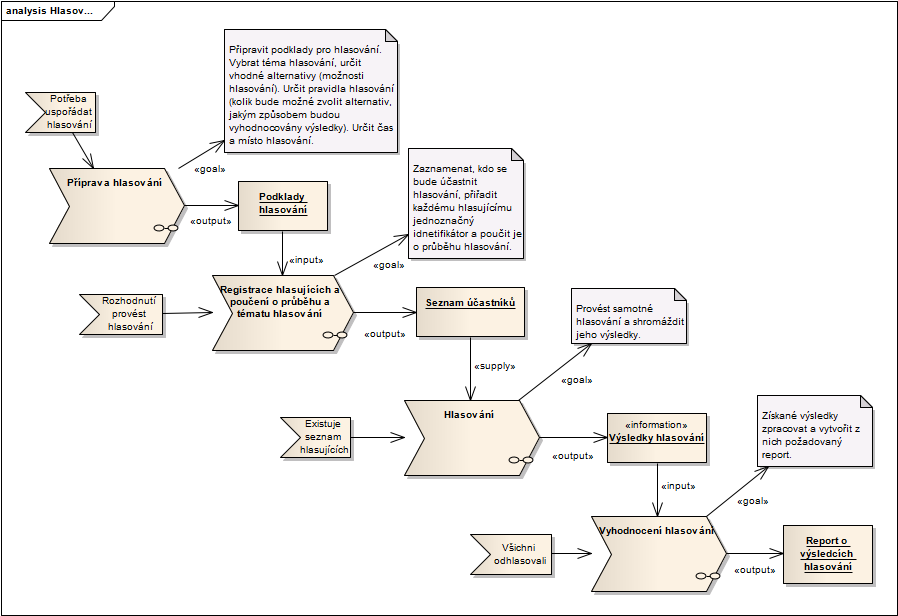
\includegraphics[width=14cm]{figures/VotingCZECH}
\caption{Business process model of voting, model by Jakub Valenta}
\label{fig:businessMOD}
\end{center}
\end{figure}

%*****************************************************************************
\chapter{Installation and how to use}
\textbf{\large Tato příloha velmi žádoucí zejména u softwarových implementačních prací.}

%*****************************************************************************
\chapter{Enclosed CD Table of Contents}
\textbf{\large Tato příloha je povinná pro každou práci. Každá práce musí totiž obsahovat přiložené CD. Viz dále.}

Může vypadat například takto. Váš seznam samozřejmě bude odpovídat typu vaší práce. (viz \cite{infodp}):

\begin{figure}[h]
\begin{center}
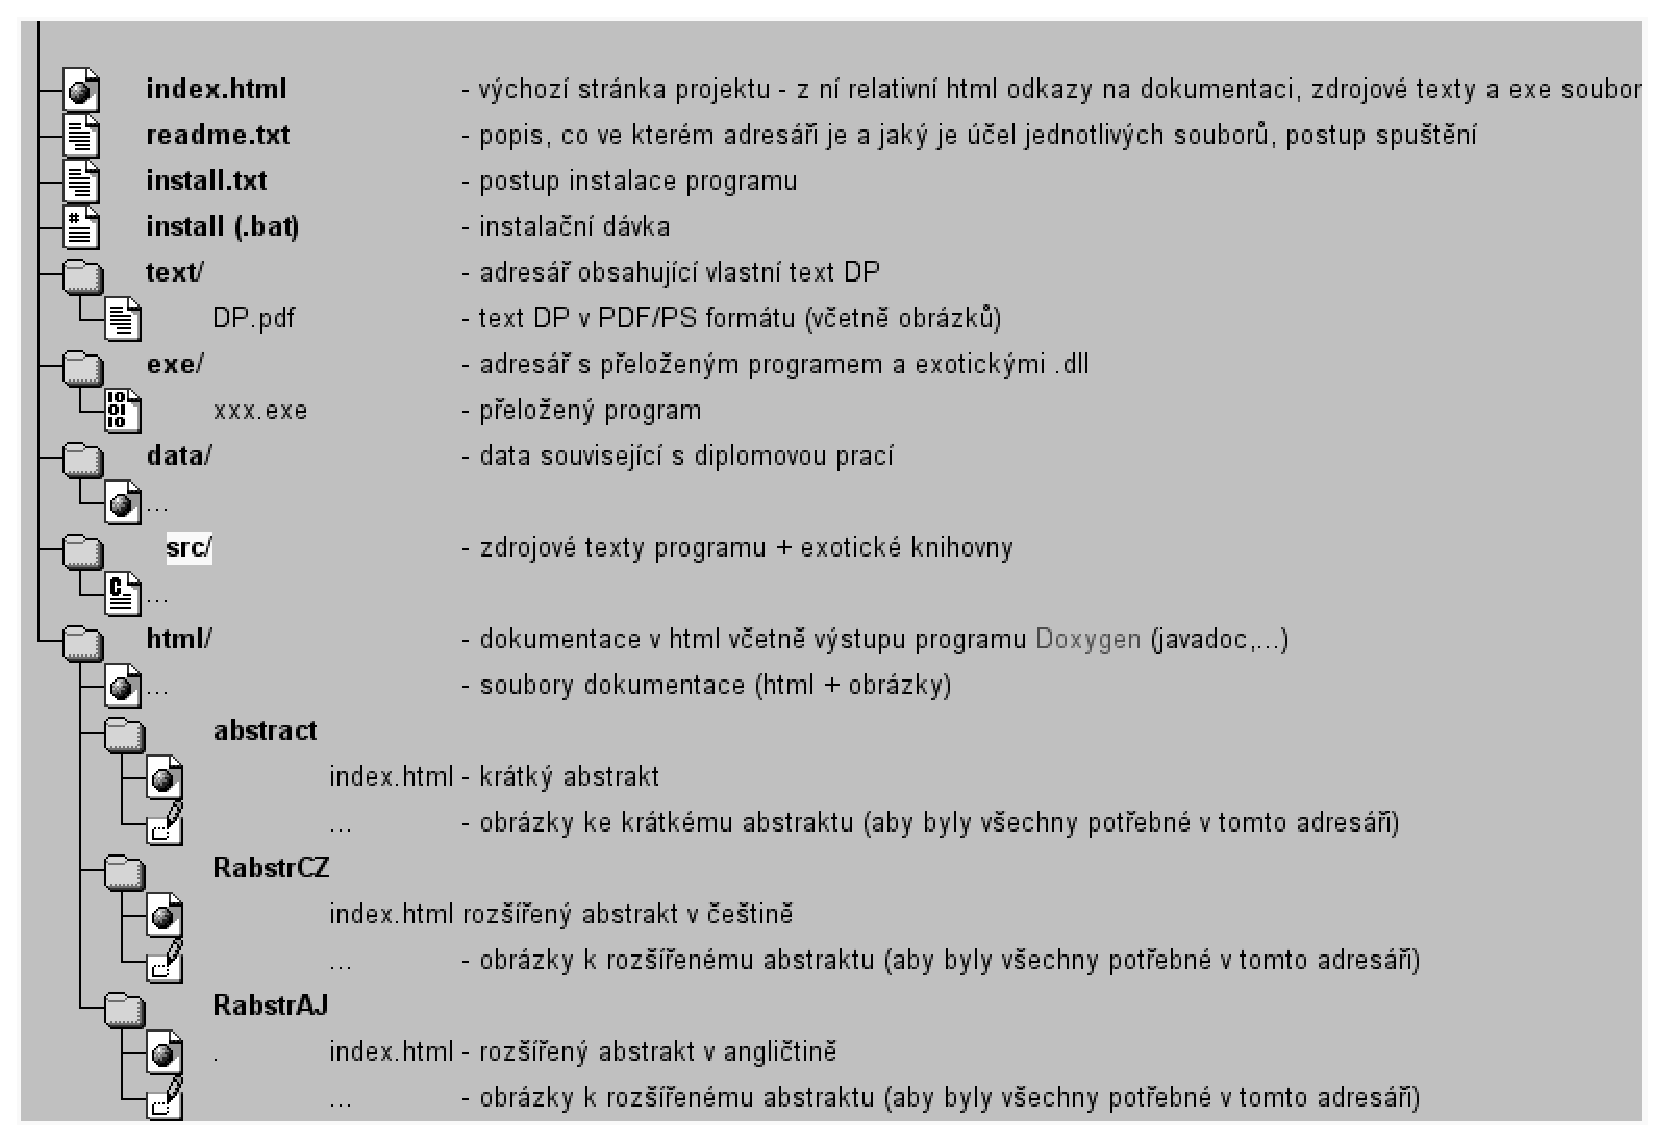
\includegraphics[width=14cm]{figures/seznamcd}
\caption{Seznam přiloženého CD --- příklad}
\label{fig:seznamcd}
\end{center}
\end{figure}



Na GNU/Linuxu si strukturu přiloženého CD můžete snadno vyrobit příkazem:\\ 
\verb|$ tree . >tree.txt|\\
Ve vzniklém souboru pak stačí pouze doplnit komentáře.

Z \textbf{README.TXT} (případne index.html apod.)  musí být rovněž zřejmé, jak programy instalovat, spouštět a jaké požadavky mají tyto programy na hardware.

Adresář \textbf{text}  musí obsahovat soubor s vlastním textem práce v PDF nebo PS formátu, který bude později použit pro prezentaci diplomové práce na WWW.

\end{document}
